% The output update as a cycle through the slice invariant, drawn like the states of
% fig:phases (noninterference.v: service_gated; model_sliced.v: initiate_next_gated).
% Proof.tex inputs this file just before V-B.
\begin{figure}[t]
\centering
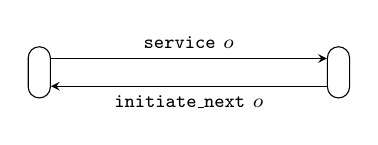
\begin{tikzpicture}[font=\scriptsize, >=stealth,
  pred/.style={draw, rounded corners, font=\small, minimum height=0.65cm, inner xsep=4pt}]
\node[pred] (g) at (0,0) {$\Gated$};
\node[pred] (b) at (3.8,0) {$\GatedB$};
\draw[->] ([yshift=5pt]g.east) -- node[above]{\texttt{service} $o$} ([yshift=5pt]b.west);
\draw[->] ([yshift=-5pt]b.west) -- node[below]{\texttt{initiate\_next} $o$} ([yshift=-5pt]g.east);
\end{tikzpicture}
\caption{The output update $g$ on output $o$, through the slice invariant
  (\cref{def:gated}). $\GatedB$ gives \m{initiate_next} the fact of \cref{def:ready}
  (\cref{lem:ready}), on which it is non-interfering (\m{initiate_next_NI_on}).}
\label{fig:lane}
\end{figure}
